% ============================================================
%  يُترجَم بـ XeLaTeX  (في Overleaf: Menu → Compiler → XeLaTeX)
%  الخط: Amiri (متوفر في Overleaf، أو حمّله من github.com/aliftype/amiri)
% ============================================================
\documentclass[12pt,a4paper]{article}
\usepackage[a4paper,margin=1.7cm,top=2.3cm,bottom=2.9cm,headheight=15pt,footskip=1.5cm]{geometry}
\usepackage{amsmath,amssymb}
\usepackage{icomma}
\usepackage[english,bidi=default,layout=lists]{babel}
\babelprovide[import,main]{arabic}
\babelfont{rm}[Scale=1.08]{Amiri}
\babelfont{sf}[Scale=1.08]{Amiri}
\usepackage[most]{tcolorbox}
\usepackage{tikz}
\usetikzlibrary{arrows.meta,calc,shadings}
\usepackage{array}
\usepackage{colortbl}
\usepackage{fancyhdr}
\usepackage{titlesec}
\usepackage{enumitem}
\usepackage{collcell}
\usepackage{needspace}
\usepackage{etoolbox}
% أعمدة جداول تُكتب خلاياها بالعربية في الاتجاه الصحيح
\newcolumntype{C}{>{\collectcell\ar}c<{\endcollectcell}}
% تجنب عنوان يتيم في أسفل الصفحة
\pretocmd{\section}{\Needspace{15\baselineskip}}{}{}
\pretocmd{\subsection}{\Needspace{11\baselineskip}}{}{}

% ---------- الألوان ----------
\definecolor{cDef}{HTML}{1F4E9C}
\definecolor{cThm}{HTML}{B3261E}
\definecolor{cRem}{HTML}{2E7D32}
\definecolor{cEx}{HTML}{C76B00}
\definecolor{cMeth}{HTML}{6A1B9A}
\definecolor{cSol}{HTML}{00695C}
\definecolor{cSec}{HTML}{1F3A68}

% ---------- العناوين ----------
\titleformat{\section}{\Large\bfseries\color{cSec}}{\thesection.}{0.6em}{}[{\color{cSec!60}\titlerule[1pt]}]
\titleformat{\subsection}{\large\bfseries\color{cThm!85!black}}{\thesubsection.}{0.5em}{}
\titlespacing*{\section}{0pt}{14pt}{8pt}
\titlespacing*{\subsection}{0pt}{10pt}{5pt}
\setlength{\parindent}{0pt}
\setlength{\parskip}{4pt}
\setlist{itemsep=2pt,topsep=3pt}

% ---------- الصناديق (تُرسم في سياق LTR ويُكتب محتواها بالعربية) ----------
\newtcolorbox{arbox}[3][]{enhanced,
  colback=#2!5,colframe=#2!80!black,arc=2mm,boxrule=0.8pt,
  left=6pt,right=6pt,top=8pt,bottom=5pt,
  fonttitle=\bfseries,coltitle=white,
  title={\foreignlanguage{arabic}{#3}},
  attach boxed title to top right={xshift=-5mm,yshift=-3mm},
  boxed title style={colback=#2!80!black,arc=1.5mm,boxrule=0pt},
  before upper={\selectlanguage{arabic}},
  before skip=8pt,after skip=8pt,breakable,#1}
\newenvironment{BOX}[2]{\begin{otherlanguage}{english}\begin{arbox}{#1}{#2}}{\end{arbox}\end{otherlanguage}}
\newenvironment{tarif}[1][تعريف]{\begin{BOX}{cDef}{#1}}{\end{BOX}}
\newenvironment{khassia}[1][خاصية]{\begin{BOX}{cThm}{#1}}{\end{BOX}}
\newenvironment{molahada}[1][ملاحظة]{\begin{BOX}{cRem}{#1}}{\end{BOX}}
\newenvironment{mithal}[1][مثال]{\begin{BOX}{cEx}{#1}}{\end{BOX}}
\newenvironment{tariqa}[1][طريقة]{\begin{BOX}{cMeth}{#1}}{\end{BOX}}

% ---------- التمارين والحلول ----------
\newcounter{exo}
\newenvironment{tamrin}[1]{\stepcounter{exo}\begin{BOX}{cSec}{التمرين \theexo: #1}}{\end{BOX}}
\newenvironment{hal}{\Needspace{12\baselineskip}\begin{otherlanguage}{english}\begin{arbox}[breakable]{cSol}{حل التمرين \theexo}}{\end{arbox}\end{otherlanguage}}

% رسومات TikZ تُوضع في سياق LTR
\newenvironment{LTR}{\begin{otherlanguage}{english}}{\end{otherlanguage}}
\newcommand{\ar}[1]{\foreignlanguage{arabic}{#1}}

% ---------- رموز ----------
% نقاط الحذف داخل الرياضيات (\dots يسبب خللاً في الاتجاه مع babel)
\renewcommand{\dots}{\mathinner{\ldotp\ldotp\ldotp}}
\renewcommand{\ldots}{\mathinner{\ldotp\ldotp\ldotp}}
\renewcommand{\cdots}{\mathinner{\cdotp\cdotp\cdotp}}
\newcommand{\N}{\mathbb{N}}
\newcommand{\Z}{\mathbb{Z}}
\newcommand{\D}{\mathbb{D}}
\newcommand{\Q}{\mathbb{Q}}
\newcommand{\R}{\mathbb{R}}
\newcommand{\pgcd}{\operatorname{PGCD}}
\newcommand{\ppcm}{\operatorname{PPCM}}

% ---------- تمثيل مجال على مستقيم عددي ----------
% \NLseg{a}{b}{[}{]}  مجال محدود
\newcommand{\NLseg}[4]{\begin{LTR}\begin{tikzpicture}[baseline=-0.6ex]
 \draw[-{Stealth[length=2mm]},gray!70](0,0)--(3.4,0);
 \draw[line width=2pt,cThm!80!black](0.7,0)--(2.7,0);
 \node[cThm!80!black,font=\LARGE] at (0.7,0){$#3$};
 \node[cThm!80!black,font=\LARGE] at (2.7,0){$#4$};
 \node[below=3pt,font=\footnotesize] at (0.7,0){$#1$};
 \node[below=3pt,font=\footnotesize] at (2.7,0){$#2$};
\end{tikzpicture}\end{LTR}}
% \NLright{a}{[}  مجال نحو +∞
\newcommand{\NLright}[2]{\begin{LTR}\begin{tikzpicture}[baseline=-0.6ex]
 \draw[-{Stealth[length=2mm]},gray!70](0,0)--(3.4,0);
 \draw[line width=2pt,cThm!80!black](1.3,0)--(3.3,0);
 \node[cThm!80!black,font=\LARGE] at (1.3,0){$#2$};
 \node[below=3pt,font=\footnotesize] at (1.3,0){$#1$};
\end{tikzpicture}\end{LTR}}
% \NLleft{b}{]}  مجال نحو −∞
\newcommand{\NLleft}[2]{\begin{LTR}\begin{tikzpicture}[baseline=-0.6ex]
 \draw[-{Stealth[length=2mm]},gray!70](0,0)--(3.4,0);
 \draw[line width=2pt,cThm!80!black](0.05,0)--(2.1,0);
 \node[cThm!80!black,font=\LARGE] at (2.1,0){$#2$};
 \node[below=3pt,font=\footnotesize] at (2.1,0){$#1$};
\end{tikzpicture}\end{LTR}}

% ---------- أيقونات مواقع التواصل (مرسومة بـ TikZ، لا تحتاج أي حزمة) ----------
\definecolor{cFB}{HTML}{1877F2}
\definecolor{cTG}{HTML}{229ED9}
\definecolor{cIG1}{HTML}{FEDA75}
\definecolor{cIG2}{HTML}{D62976}
\definecolor{cIG3}{HTML}{4F5BD5}
\newcommand{\fbicon}{\begin{LTR}\begin{tikzpicture}[baseline=-0.75ex,x=1em,y=1em]
 \fill[cFB] (0,0) circle (0.55);
 \node[white,inner sep=0,font=\usefont{TU}{lmss}{bx}{n}\small] at (0.04,-0.02) {f};
\end{tikzpicture}\end{LTR}}
\newcommand{\igicon}{\begin{LTR}
\begin{tikzpicture}[baseline=-0.75ex,x=1em,y=1em]
 \shade[lower left=cIG1,lower right=cIG2,upper left=cIG2,upper right=cIG3,rounded corners=0.28em] (-0.55,-0.55) rectangle (0.55,0.55);
 \draw[white,line width=0.09em,rounded corners=0.18em] (-0.36,-0.36) rectangle (0.36,0.36);
 \draw[white,line width=0.09em] (0,0) circle (0.17);
 \fill[white] (0.22,0.22) circle (0.05);
\end{tikzpicture}\end{LTR}}
\newcommand{\tgicon}{\begin{LTR}
\begin{tikzpicture}[baseline=-0.75ex,x=1em,y=1em]
 \fill[cTG] (0,0) circle (0.55);
 \fill[white] (-0.33,0.0) -- (0.32,0.27) -- (0.2,-0.3) -- (0.0,-0.15) -- (-0.08,-0.28) -- (-0.08,-0.08) -- cycle;
 \fill[cTG!70!black] (-0.08,-0.08) -- (0.25,0.2) -- (0.0,-0.15) -- (-0.08,-0.28) -- cycle;
\end{tikzpicture}\end{LTR}}
% سطر مواقع التواصل أسفل كل صفحة
% (يُكتب السطر بترتيب بصري من اليسار إلى اليمين: الأيقونة يمين كل اسم)
\newcommand{\PageBox}{\begin{LTR}\tikz[baseline=(p.base)]\node[fill=black,text=white,inner sep=2.5pt,minimum width=1.6em,minimum height=1.3em,font=\usefont{TU}{lmss}{bx}{n}\small](p){\ifnum\value{page}<10 0\fi\arabic{page}};\end{LTR}}
\newcommand{\SocialRow}{\begin{otherlanguage}{english}%
 \ar{\textbf{الأستاذ سوايسية هشام للرياضيات}}\ \tgicon\hfill
 \textbf{prof\_hicham\_math}\ \igicon\hfill
 \ar{\textbf{الأستاذ سوايسية هشام للرياضيات}}\ \fbicon\hspace{2.2em}\PageBox\end{otherlanguage}}
% ---------- رأس وتذييل الصفحة ----------
\pagestyle{fancy}
\fancyhf{}
\renewcommand{\headrulewidth}{0.6pt}
\renewcommand{\footrulewidth}{0.4pt}
% \SetHeader{يمين الرأس}{يسار الرأس}{يمين التذييل}{يسار التذييل}
\newcommand{\SetHeader}[2]{%
 \fancyhead[C]{\parbox{\textwidth}{\ar{#1\hfill #2}}}%
 \fancyfoot[C]{\parbox{\textwidth}{\small\SocialRow}}}

\usepackage{tkz-tab}
\usepackage{multicol}
% جدول تغيرات / إشارة (يُرسم في سياق LTR)
\newenvironment{TAB}{\par\begin{center}\begin{LTR}\begin{tikzpicture}[scale=0.95,every node/.style={font=\small}]}{\end{tikzpicture}\end{LTR}\end{center}}
% معلم بشبكة: \begin{GR}{xmin}{xmax}{ymin}{ymax}{unit cm}
\newenvironment{GR}[5]{\par\begin{center}\begin{LTR}\begin{tikzpicture}[x=#5cm,y=#5cm,font=\footnotesize]
 \def\xmn{#1}\def\xmx{#2}\def\ymn{#3}\def\ymx{#4}
 \draw[gray!25,very thin] (#1,#3) grid (#2,#4);
 \draw[-{Stealth[length=2mm]}] (#1,0)--(#2+0.3,0) node[below left]{$x$};
 \draw[-{Stealth[length=2mm]}] (0,#3)--(0,#4+0.3) node[below left]{$y$};
 \node[below left] at (0,0){$O$};
 \draw[very thick,-{Stealth[length=1.6mm]}] (0,0)--(1,0) node[below,pos=.55]{$\vec i$};
 \draw[very thick,-{Stealth[length=1.6mm]}] (0,0)--(0,1) node[left,pos=.55]{$\vec j$};
 \begin{scope}\clip (#1,#3) rectangle (#2,#4);}
{\end{scope}\end{tikzpicture}\end{LTR}\end{center}}
\newcommand{\Ticks}[2]{\foreach \t in {#1} \node[below,font=\scriptsize] at (\t,0){$\t$}; \foreach \t in {#2} \node[left,font=\scriptsize] at (0,\t){$\t$};}
\newcommand{\bx}[1]{\ensuremath{\colorbox{cDef!12}{$\displaystyle #1$}}}
\newcommand{\hl}[1]{\ensuremath{\colorbox{cEx!20}{$\displaystyle #1$}}}
\newcommand{\Lim}[1]{\displaystyle\lim_{x\to #1}}
\newcommand{\Cf}{(C_f)}
\newenvironment{qst}{\begin{enumerate}[label=\protect\circled{\arabic*},leftmargin=*]}{\end{enumerate}}
\newcommand{\circled}[1]{\foreignlanguage{english}{\tikz[baseline=(c.base)]\node[circle,fill=cDef,text=white,inner sep=1.2pt,font=\scriptsize\bfseries](c){#1};}}
% عمودان: \TwoCol{عرض اليسار}{محتوى اليسار}{عرض اليمين}{محتوى اليمين}  (آمن مع TikZ)
\newcommand{\TwoCol}[4]{\par\begin{LTR}\noindent\begin{minipage}[t]{#1\textwidth}\selectlanguage{arabic}#2\end{minipage}\hfill\begin{minipage}[t]{#3\textwidth}\selectlanguage{arabic}#4\end{minipage}\end{LTR}\par}
\newcommand{\un}{(u_n)}\newcommand{\vn}{(v_n)}
% برهان بالتراجع: \Rec{الخاصية P(n)}{التحقق من P(0)}{البرهان على الوراثة}
\newcommand{\Rec}[3]{\textbf{برهان بالتراجع:} نسمي $P(n)$ الخاصية: «#1».
\begin{itemize}
\item \textbf{التحقق:} #2
\item \textbf{الوراثة:} نفرض أن $P(n)$ صحيحة ونبرهن صحة $P(n+1)$: #3
\item \textbf{الخلاصة:} حسب مبدأ الاستدلال بالتراجع، $P(n)$ صحيحة من أجل كل عدد طبيعي $n$.
\end{itemize}}
\newcommand{\src}[1]{{\footnotesize\textbf{#1}}\par}
\newcommand{\ok}{$\textcolor{cRem}{\checkmark}$}
\newcommand{\limn}{\displaystyle\lim_{n\to+\infty}}
% أسئلة فرعية (أ) (ب) (جـ) كل سؤال في سطر
\newenvironment{sq}{\begin{itemize}[leftmargin=2.4em,itemsep=3pt]}{\end{itemize}}
\newcommand{\qa}{\item[(أ)]}\newcommand{\qb}{\item[(ب)]}\newcommand{\qc}{\item[(جـ)]}\newcommand{\qd}{\item[(د)]}\newcommand{\qe}{\item[(هـ)]}
\newcommand{\pa}{\par\smallskip\textbf{(أ)} }\newcommand{\pb}{\par\smallskip\textbf{(ب)} }\newcommand{\pc}{\par\smallskip\textbf{(جـ)} }\newcommand{\pd}{\par\smallskip\textbf{(د)} }\newcommand{\pe}{\par\smallskip\textbf{(هـ)} }
\newcommand{\ccl}[1]{\par\textbf{الخلاصة:} #1}

\pretocmd{\section}{\Needspace{24\baselineskip}}{}{}
\SetHeader{\small\bfseries\color{cSec}تمارين: الهندسة المستوية}{\small\color{cSec}السنة الأولى ثانوي -- جذع مشترك علوم وتكنولوجيا}
\begin{document}
\newcolumntype{M}[1]{>{\centering\arraybackslash}p{#1}}
\newcommand{\RL}[4]{\TwoCol{#3}{#4}{#1}{#2}}
\newcommand{\QQ}[1]{\par\smallskip\textbf{#1.} }
\newcommand{\ABC}[3]{\\[2pt]\begin{tabular}{p{0.28\textwidth}p{0.28\textwidth}p{0.28\textwidth}}(جـ) \ #3 & (ب) \ #2 & (أ) \ #1\end{tabular}}
\newcommand{\V}[1]{\overrightarrow{#1}}
\begin{LTR}
\begin{tcolorbox}[enhanced,colback=cSec,colframe=cSec,arc=3mm,halign=center,boxrule=0pt,top=12pt,bottom=12pt,before upper={\selectlanguage{arabic}}]
{\color{white}\fontsize{26}{32}\selectfont\bfseries سلسلة تمارين: الهندسة المستوية}\\[8pt]
{\color{white}\large تمارين متنوعة ونماذج فروض مع الحلول المفصلة والأشكال}\\[5pt]
{\color{white}\large السنة الأولى ثانوي -- جذع مشترك علوم وتكنولوجيا}
\end{tcolorbox}
\end{LTR}

% =====================================================================
\section{فيثاغورس ، طالس والمستقيمات الخاصة}
% ------------------------------------------------- 1
\begin{tamrin}{مثلث قائم داخل مربع}
\RL{0.6}{%
$ABCD$ مربع طول ضلعه $10\,cm$ ، $N$ منتصف $[BC]$ ، و $M$ نقطة من $[DC]$ حيث $AM=\dfrac{25}{2}\,cm$.
\begin{enumerate}
\item أنشئ الشكل ، واحسب الطول $DM$.
\item ما نوع المثلث $ANM$؟ برّر إجابتك.
\item $H$ المسقط العمودي للنقطة $N$ على $[AM]$. احسب $NH$.
\end{enumerate}}{0.37}{%
\begin{LTR}\centering
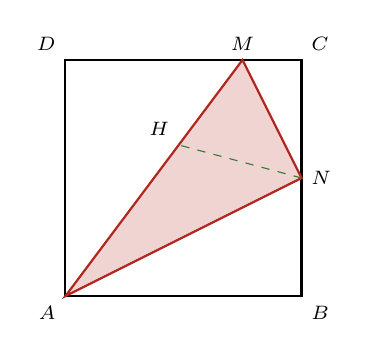
\begin{tikzpicture}[scale=0.3,font=\scriptsize]
\coordinate (A) at (0,0); \coordinate (B) at (10,0); \coordinate (C) at (10,10); \coordinate (D) at (0,10);
\coordinate (N) at (10,5); \coordinate (M) at (7.5,10);
\draw[thick] (A)--(B)--(C)--(D)--cycle;
\fill[cThm!20] (A)--(N)--(M)--cycle; \draw[cThm,thick] (A)--(N)--(M)--cycle;
\coordinate (H) at ($(A)!0.64!(M)$); \draw[cRem,dashed] (N)--(H);
\node[below left] at (A){$A$}; \node[below right] at (B){$B$}; \node[above right] at (C){$C$}; \node[above left] at (D){$D$};
\node[right] at (N){$N$}; \node[above] at (M){$M$}; \node[above left] at (H){$H$};
\end{tikzpicture}
\end{LTR}}
\end{tamrin}
\begin{hal}
\textbf{1.} المثلث $ADM$ قائم في $D$: $DM^2=AM^2-AD^2=156{,}25-100=56{,}25$ ، \ \bx{DM=7{,}5\,cm} ، ومنه $MC=2{,}5\,cm$.
\QQ{2} فيثاغورس:
\begin{itemize}
\item في $ABN$ القائم في $B$: $AN^2=10^2+5^2=125$.
\item في $NCM$ القائم في $C$: $NM^2=5^2+2{,}5^2=31{,}25$.
\end{itemize}
$AN^2+NM^2=125+31{,}25=156{,}25=AM^2$: حسب عكس فيثاغورس \textbf{$ANM$ قائم في $N$}.
\QQ{3} مساحة المثلث $ANM$ تُحسب بطريقتين: $\dfrac{AN\times NM}{2}=\dfrac{AM\times NH}{2}$ ، إذن:
\[NH=\frac{AN\times NM}{AM}=\frac{\sqrt{125}\times\sqrt{31{,}25}}{12{,}5}=\frac{\sqrt{3906{,}25}}{12{,}5}=\frac{62{,}5}{12{,}5}=\bx{5\,cm}.\]
\end{hal}

% ------------------------------------------------- 2
\begin{tamrin}{وتر في دائرة}
لتكن $(C)$ دائرة مركزها $O$ ونصف قطرها $r=5$ ، و $[AB]$ وتر فيها ، و $H$ المسقط العمودي للنقطة $O$ على $[AB]$ حيث $OH=3$.
\begin{enumerate}
\item أنشئ الشكل. ما نوع المثلث $OAB$؟ علّل.
\item احسب طول الوتر $[AB]$.
\item لتكن $E$ نظيرة $A$ بالنسبة إلى $O$. ما نوع المثلث $ABE$؟ علّل ، ثم احسب $BE$.
\item لتكن $K$ منتصف القطعة $[BE]$. أثبت أن المثلثين $KOH$ و $ABE$ متشابهان مع تعيين نسبة التشابه.
\end{enumerate}
\end{tamrin}
\begin{hal}
\RL{0.6}{%
\textbf{1.} $OA=OB=r=5$: \ \textbf{$OAB$ متساوي الساقين رأسه $O$}.
\QQ{2} في $OAH$ القائم في $H$: $AH^2=25-9=16$ ، $AH=4$. \ في المثلث متساوي الساقين الارتفاع $[OH]$ متوسط أيضاً ، فـ $H$ منتصف $[AB]$: \ \bx{AB=8}.
\QQ{3} $[AE]$ قطر و $B$ على الدائرة: \ \textbf{$ABE$ قائم في $B$}. \ $BE^2=AE^2-AB^2=100-64=36$ ، \bx{BE=6}.}{0.37}{%
\begin{LTR}\centering
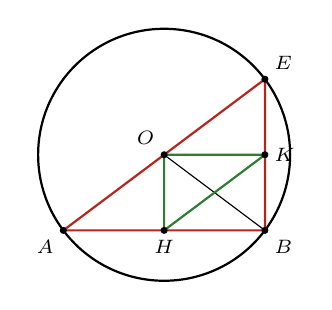
\begin{tikzpicture}[scale=0.32,font=\scriptsize]
\coordinate (O) at (0,0); \coordinate (A) at (-4,-3); \coordinate (B) at (4,-3); \coordinate (E) at (4,3);
\coordinate (H) at (0,-3); \coordinate (K) at (4,0);
\draw[thick] (O) circle (5);
\draw[cThm,thick] (A)--(B)--(E)--cycle; \draw (O)--(B) (O)--(H); \draw[cRem,thick] (O)--(K)--(H)--cycle;
\foreach \p/\n/\a in {O/O/above left,A/A/below left,B/B/below right,E/E/above right,H/H/below,K/K/right} \fill (\p) circle (4pt) node[\a]{$\n$};
\end{tikzpicture}
\end{LTR}}
\QQ{4} في المثلث $ABE$: $O$ منتصف $[AE]$ ، $H$ منتصف $[AB]$ و $K$ منتصف $[BE]$. \ حسب مستقيم المنتصفين:
\[OH=\frac{BE}2=3\quad;\quad OK=\frac{AB}2=4\quad;\quad HK=\frac{AE}2=5.\]
الأطوال متناسبة: $\dfrac{OH}{BE}=\dfrac{OK}{AB}=\dfrac{HK}{AE}=\dfrac12$: \ المثلثان \textbf{متشابهان} بنسبة \bx{k=\dfrac12}.
\end{hal}

% ------------------------------------------------- 3
\begin{tamrin}{شبه منحرف قائم}
\RL{0.55}{%
$ABCD$ شبه منحرف قائم قاعدتاه $[AD]$ و $[BC]$ حيث $AD=3\,cm$ و $BC=4\,cm$ (الزاويتان $\widehat C$ و $\widehat D$ قائمتان). \ المستقيم $(AB)$ يقطع $(DC)$ في $O$ حيث $OD=21\,cm$ ، و $E$ نقطة من $[DC]$ حيث $EC=3\,cm$.
\begin{enumerate}
\item احسب $DC$ ، ثم مساحة شبه المنحرف $ABCD$.
\item بيّن أن الزاوية $\widehat{AEB}$ قائمة ، ثم احسب الطول $AB$.
\item أثبت أن المثلثين $OAD$ و $OBC$ متشابهان ، واحسب نسبة تشابههما.
\item احسب قيسي الزاويتين $\widehat{EAB}$ و $\widehat{EBA}$.
\item هل النقط $A$ ، $B$ ، $C$ و $D$ تنتمي إلى نفس الدائرة؟ علّل.
\end{enumerate}}{0.42}{%
\begin{LTR}\centering
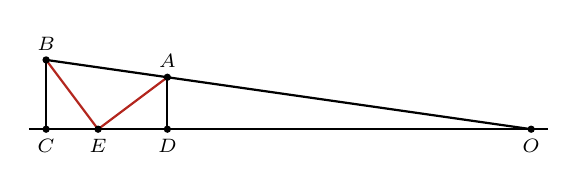
\begin{tikzpicture}[scale=0.22,font=\scriptsize]
\coordinate (C) at (0,0); \coordinate (B) at (0,4); \coordinate (D) at (7,0); \coordinate (A) at (7,3); \coordinate (E) at (3,0); \coordinate (O) at (28,0);
\draw[thick] (-1,0)--(29,0); \draw[thick] (B)--(O);
\draw[thick] (C)--(B) (D)--(A); \draw[cThm,thick] (B)--(E)--(A);
\foreach \p/\n/\a in {C/C/below,B/B/above,D/D/below,A/A/above,E/E/below,O/O/below} \fill (\p) circle (6pt) node[\a]{$\n$};
\end{tikzpicture}
\end{LTR}}
\end{tamrin}
\begin{hal}
\textbf{1.} $(AD)\parallel(BC)$ (كلاهما عمودي على $(DC)$) ، وحسب طالس في المثلث $OBC$: $\dfrac{OD}{OC}=\dfrac{AD}{BC}=\dfrac34$ ، إذن $OC=\dfrac{4\times21}{3}=28$ و \bx{DC=28-21=7\,cm}.\par
المساحة: $\dfrac{(AD+BC)\times DC}{2}=\dfrac{(3+4)\times7}{2}=\bx{24{,}5\,cm^2}$.
\QQ{2} $ED=DC-EC=4$. \ في $AED$ القائم في $D$: $AE^2=9+16=25$ ، $AE=5$. \ في $BEC$ القائم في $C$: $BE^2=16+9=25$ ، $BE=5$.\par
المثلثان $AED$ و $EBC$ متقايسان (الحالة ض ز ض: $ED=BC=4$ ، $AD=EC=3$ ، والزاويتان قائمتان) ، إذن $\widehat{DAE}=\widehat{CEB}$ ، ومنه:
\[\widehat{AED}+\widehat{BEC}=\widehat{AED}+\widehat{DAE}=90^\circ\ \Rightarrow\ \widehat{AEB}=180^\circ-90^\circ=\bx{90^\circ}.\]
$AB^2=AE^2+BE^2=50$ ، \ \bx{AB=5\sqrt2\,cm}.
\QQ{3} للمثلثين $OAD$ و $OBC$ الزاوية $\widehat O$ مشتركة ، و $\widehat{ODA}=\widehat{OCB}=90^\circ$: \textbf{متشابهان} ، ونسبة التشابه \bx{k=\dfrac{OD}{OC}=\dfrac{21}{28}=\dfrac34}.
\QQ{4} $ABE$ قائم في $E$ و $AE=BE$: متساوي الساقين ، إذن \bx{\widehat{EAB}=\widehat{EBA}=45^\circ}.
\QQ{5} \textbf{لا:} لو كانت على دائرة واحدة لكان $[AC]$ قطراً لها (لأن $\widehat{ADC}=90^\circ$) ، ولكانت $\widehat{ABC}=90^\circ$ ، وهذا خطأ لأن $(AB)$ ليس موازياً لـ $(DC)$ ($AD\ne BC$).
\end{hal}

% ------------------------------------------------- 4
\begin{tamrin}{مثلث متساوي الساقين ومنتصف ارتفاع}
$ABC$ مثلث متساوي الساقين رأسه $A$ حيث $AB=AC=4\,cm$ و $BC=6\,cm$. \ $H$ المسقط العمودي للنقطة $A$ على $(BC)$ ، $E$ منتصف $[AC]$ و $F$ مسقطها العمودي على $(AH)$.
\begin{enumerate}
\item أنجز شكلاً مناسباً.
\item بيّن أن $F$ منتصف القطعة $[AH]$.
\item احسب الأطوال $AH$ ، $AF$ و $FE$.
\item لتكن $G$ نقطة من $[AB]$ حيث $AG=AE$.
\begin{sq}
\qa بيّن أن المثلثين $AGE$ و $ABC$ متشابهان ، وعيّن نسبة التشابه.
\qb أثبت أن المثلثين $GBC$ و $ECB$ متقايسان.
\qc ما طبيعة الرباعي $HFEC$؟ احسب مساحته.
\end{sq}
\end{enumerate}
\end{tamrin}
\begin{hal}
\RL{0.6}{%
\textbf{2.} $(EF)\perp(AH)$ و $(CH)\perp(AH)$ ، إذن $(EF)\parallel(CH)$. \ في المثلث $AHC$: $E$ منتصف $[AC]$ و $(EF)\parallel(HC)$ ، فحسب مستقيم المنتصفين (أو طالس: $\dfrac{AF}{AH}=\dfrac{AE}{AC}=\dfrac12$): \ \textbf{$F$ منتصف $[AH]$}.
\QQ{3} الارتفاع في المثلث متساوي الساقين متوسط أيضاً: $HC=3$. \ $AH^2=16-9=7$ ، \bx{AH=\sqrt7\,cm} ، \ \bx{AF=\dfrac{\sqrt7}2\,cm} ، و \bx{FE=\dfrac{HC}{2}=1{,}5\,cm}.}{0.37}{%
\begin{LTR}\centering
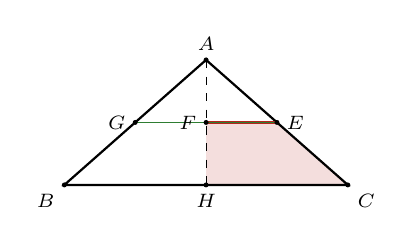
\begin{tikzpicture}[scale=0.6,font=\scriptsize]
\coordinate (B) at (-3,0); \coordinate (C) at (3,0); \coordinate (A) at (0,2.6458); \coordinate (H) at (0,0);
\coordinate (E) at (1.5,1.3229); \coordinate (F) at (0,1.3229); \coordinate (G) at (-1.5,1.3229);
\fill[cThm!15] (H)--(F)--(E)--(C)--cycle;
\draw[thick] (A)--(B)--(C)--cycle; \draw[dashed] (A)--(H); \draw[cThm,thick] (F)--(E); \draw[cRem] (G)--(E);
\foreach \p/\n/\a in {A/A/above,B/B/below left,C/C/below right,H/H/below,E/E/right,F/F/left,G/G/left} \fill (\p) circle (1.5pt) node[\a]{$\n$};
\end{tikzpicture}
\end{LTR}}
\QQ{4}
\begin{sq}
\qa $AG=AE=2$: \ $\dfrac{AG}{AB}=\dfrac{AE}{AC}=\dfrac12$ والزاوية $\widehat A$ مشتركة: \ \textbf{متشابهان} بنسبة \bx{\dfrac12}.
\qb $GB=4-2=2=EC$ ، $[BC]$ ضلع مشترك ، و $\widehat{GBC}=\widehat{ECB}$ (زاويتا القاعدة): الحالة \textbf{(ض ، ز ، ض)} ، إذن \textbf{متقايسان}.
\qc $(FE)\parallel(HC)$ و $(FH)\perp(HC)$: \ \textbf{$HFEC$ شبه منحرف قائم}. \ مساحته:
\[\frac{(FE+HC)\times FH}{2}=\frac{(1{,}5+3)\times\frac{\sqrt7}{2}}{2}=\bx{\frac{9\sqrt7}{8}\,cm^2}\approx2{,}98\,cm^2.\]
\end{sq}
\end{hal}

% =====================================================================
\section{المثلثات المتقايسة والمتشابهة}
% ------------------------------------------------- 5
\begin{tamrin}{مثلث متقايس الأضلاع ومثلث داخلي}
\RL{0.58}{%
$ABC$ مثلث متقايس الأضلاع طول ضلعه $3\,cm$. \ $D$ ، $E$ و $F$ نقط من $[AB]$ ، $[BC]$ و $[CA]$ على الترتيب حيث: $AD=BE=CF=1\,cm$.
\begin{enumerate}
\item أنشئ الشكل المطلوب.
\item بيّن أن المثلثات $ADF$ ، $BED$ و $CFE$ متقايسة ، ثم استنتج نوع المثلث $DEF$.
\item استنتج أن المثلثين $ABC$ و $DEF$ متشابهان.
\item لتكن $H$ نقطة من $[BC]$ بحيث يكون $(AH)$ محور القطعة $[BC]$. \ أثبت أن $(AH)\parallel(DE)$ (استعمل عكس طالس).
\item استنتج أن المثلث $BDE$ قائم في $E$ ، ثم احسب الطول $ED$.
\end{enumerate}}{0.39}{%
\begin{LTR}\centering
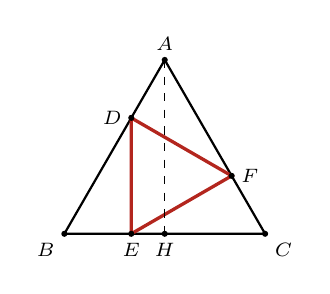
\begin{tikzpicture}[scale=0.85,font=\scriptsize]
\coordinate (B) at (0,0); \coordinate (C) at (3,0); \coordinate (A) at (1.5,2.598);
\coordinate (D) at ($(A)!1/3!(B)$); \coordinate (E) at ($(B)!1/3!(C)$); \coordinate (F) at ($(C)!1/3!(A)$); \coordinate (H) at (1.5,0);
\draw[thick] (A)--(B)--(C)--cycle; \draw[cThm,very thick] (D)--(E)--(F)--cycle; \draw[dashed] (A)--(H);
\foreach \p/\n/\a in {A/A/above,B/B/below left,C/C/below right,D/D/left,E/E/below,F/F/right,H/H/below} \fill (\p) circle (1.3pt) node[\a]{$\n$};
\end{tikzpicture}
\end{LTR}}
\end{tamrin}
\begin{hal}
\textbf{2.} $AF=AC-CF=2$ ، $BD=AB-AD=2$ ، $CE=BC-BE=2$. \ في المثلثات الثلاثة:
\[AD=BE=CF=1\quad;\quad AF=BD=CE=2\quad;\quad\widehat A=\widehat B=\widehat C=60^\circ.\]
الحالة \textbf{(ض ، ز ، ض)}: المثلثات \textbf{متقايسة} ، ومنه $DF=ED=FE$: \ \textbf{$DEF$ متقايس الأضلاع}.
\QQ{3} زوايا المثلثين $ABC$ و $DEF$ كلها $60^\circ$: \textbf{متشابهان}.
\QQ{4} $(AH)$ محور $[BC]$ ، إذن $H$ منتصف $[BC]$ و $BH=1{,}5$.\par
$\dfrac{BE}{BH}=\dfrac{1}{1{,}5}=\dfrac23$ و $\dfrac{BD}{BA}=\dfrac23$ ، والنقط $B,E,H$ و $B,D,A$ بنفس الترتيب: حسب عكس طالس \bx{(DE)\parallel(AH)}.
\QQ{5} $(AH)\perp(BC)$ و $(DE)\parallel(AH)$ ، إذن $(DE)\perp(BC)$: \textbf{$BDE$ قائم في $E$}.\par
$ED^2=BD^2-BE^2=4-1=3$ ، \ \bx{ED=\sqrt3\,cm} \ (وهو طول ضلع المثلث $DEF$).
\end{hal}

% ------------------------------------------------- 6
\begin{tamrin}{منتصفات أضلاع مثلث متساوي الساقين}
\RL{0.58}{%
$ABC$ مثلث متساوي الساقين رأسه $A$ حيث $AC=5\,cm$ و $BC=8\,cm$. \ $E$ ، $F$ و $G$ منتصفات $[AB]$ ، $[AC]$ و $[BC]$ على الترتيب.
\begin{enumerate}
\item بيّن أن المثلثين $AEF$ و $ABC$ متشابهان ، ثم عيّن نسبة التشابه.
\item بيّن أن المثلثين $FCG$ و $EBG$ متقايسان.
\item احسب الطول $AG$ ، وبيّن أن المستقيمين $(AC)$ و $(EG)$ متوازيان.
\end{enumerate}}{0.39}{%
\begin{LTR}\centering
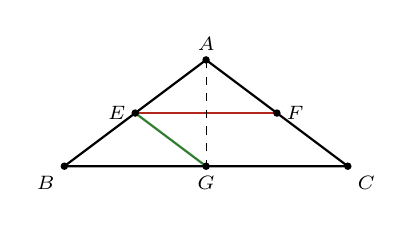
\begin{tikzpicture}[scale=0.45,font=\scriptsize]
\coordinate (B) at (0,0); \coordinate (C) at (8,0); \coordinate (A) at (4,3);
\coordinate (E) at (2,1.5); \coordinate (F) at (6,1.5); \coordinate (G) at (4,0);
\draw[thick] (A)--(B)--(C)--cycle; \draw[cThm,thick] (E)--(F); \draw[cRem,thick] (E)--(G); \draw[dashed] (A)--(G);
\foreach \p/\n/\a in {A/A/above,B/B/below left,C/C/below right,E/E/left,F/F/right,G/G/below} \fill (\p) circle (3pt) node[\a]{$\n$};
\end{tikzpicture}
\end{LTR}}
\end{tamrin}
\begin{hal}
\textbf{1.} $\dfrac{AE}{AB}=\dfrac{AF}{AC}=\dfrac12$ والزاوية $\widehat A$ مشتركة: \ \textbf{متشابهان} بنسبة \bx{\dfrac12} \ (و $EF=\dfrac{BC}2=4$).
\QQ{2} $FC=EB=2{,}5$ ، $CG=BG=4$ ، و $\widehat C=\widehat B$ (زاويتا القاعدة): الحالة \textbf{(ض ، ز ، ض)}: \textbf{متقايسان}.
\QQ{3} المتوسط $[AG]$ ارتفاع أيضاً: $AG^2=AC^2-GC^2=25-16=9$ ، \ \bx{AG=3\,cm}.\par
في المثلث $ABC$: $E$ منتصف $[AB]$ و $G$ منتصف $[BC]$ ، فحسب مستقيم المنتصفين \bx{(EG)\parallel(AC)}.
\end{hal}

% ------------------------------------------------- 7
\begin{tamrin}{الارتفاع المتعلق بالوتر}
\RL{0.6}{%
$ABC$ مثلث قائم في $A$ ومتساوي الساقين ، و $H$ المسقط العمودي للنقطة $A$ على $[BC]$.
\begin{enumerate}
\item برهن أن المثلثين $ABC$ و $HAB$ متشابهان.
\item عيّن نسبة التشابه الذي يحوّل المثلث $ABC$ إلى المثلث $HAB$.
\item احسب النسبة $\dfrac{S_{HAB}}{S_{ABC}}$ حيث $S_{HAB}$ و $S_{ABC}$ مساحتا المثلثين.
\end{enumerate}}{0.37}{%
\begin{LTR}\centering
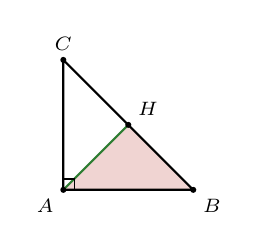
\begin{tikzpicture}[scale=0.55,font=\scriptsize]
\coordinate (A) at (0,0); \coordinate (B) at (3,0); \coordinate (C) at (0,3); \coordinate (H) at (1.5,1.5);
\fill[cThm!20] (A)--(B)--(H)--cycle;
\draw[thick] (A)--(B)--(C)--cycle; \draw[cRem,thick] (A)--(H);
\draw (0.25,0)--(0.25,0.25)--(0,0.25);
\foreach \p/\n/\a in {A/A/below left,B/B/below right,C/C/above,H/H/above right} \fill (\p) circle (2pt) node[\a]{$\n$};
\end{tikzpicture}
\end{LTR}}
\end{tamrin}
\begin{hal}
\textbf{1.} للمثلثين $ABC$ و $HAB$ الزاوية $\widehat B$ مشتركة ، و $\widehat{BAC}=\widehat{AHB}=90^\circ$: لهما زاويتان متقايستان ، إذن \textbf{متشابهان}.
\QQ{2} الضلع المقابل للزاوية القائمة في $ABC$ هو $BC$ ، وفي $HAB$ هو $AB$. \ مع $BC=AB\sqrt2$:
\[k=\frac{AB}{BC}=\frac{AB}{AB\sqrt2}=\bx{\frac{\sqrt2}{2}}.\]
\QQ{3} $\dfrac{S_{HAB}}{S_{ABC}}=k^2=\bx{\dfrac12}$ \ (وهذا منطقي: $H$ منتصف $[BC]$ والمتوسط يقسم المثلث إلى مثلثين لهما نفس المساحة).
\end{hal}

% ------------------------------------------------- 8
\begin{tamrin}{مربع ومثلثان متشابهان}
$ABCD$ مربع طول ضلعه $a$ ($a>0$) ، $M$ منتصف $[DC]$ ، و $N$ نقطة من المستوي حيث $\V{CN}=\dfrac14\V{CB}$.
\begin{enumerate}
\item أنجز الشكل.
\item احسب بدلالة $a$ الأطوال $AM$ ، $MN$ و $AN$.
\item بيّن أن المثلث $AMN$ قائم.
\item بيّن أن المثلثين $ADM$ و $MCN$ متشابهان ، ثم عيّن نسبة التشابه.
\end{enumerate}
\end{tamrin}
\begin{hal}
\RL{0.62}{%
\textbf{2.} $DM=MC=\dfrac a2$ ، $CN=\dfrac a4$ ، $NB=\dfrac{3a}4$.
\begin{itemize}
\item $AM^2=AD^2+DM^2=a^2+\dfrac{a^2}4=\dfrac{5a^2}4$: \ \bx{AM=\dfrac{a\sqrt5}2}.
\item $MN^2=MC^2+CN^2=\dfrac{a^2}4+\dfrac{a^2}{16}=\dfrac{5a^2}{16}$: \ \bx{MN=\dfrac{a\sqrt5}4}.
\item $AN^2=AB^2+BN^2=a^2+\dfrac{9a^2}{16}=\dfrac{25a^2}{16}$: \ \bx{AN=\dfrac{5a}4}.
\end{itemize}}{0.35}{%
\begin{LTR}\centering
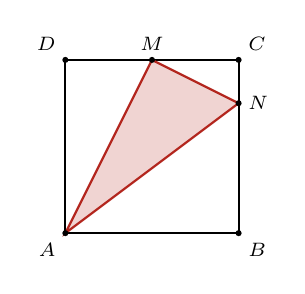
\begin{tikzpicture}[scale=0.55,font=\scriptsize]
\coordinate (A) at (0,0); \coordinate (B) at (4,0); \coordinate (C) at (4,4); \coordinate (D) at (0,4); \coordinate (M) at (2,4); \coordinate (N) at (4,3);
\draw[thick] (A)--(B)--(C)--(D)--cycle; \fill[cThm!20] (A)--(M)--(N)--cycle; \draw[cThm,thick] (A)--(M)--(N)--cycle;
\foreach \p/\n/\a in {A/A/below left,B/B/below right,C/C/above right,D/D/above left,M/M/above,N/N/right} \fill (\p) circle (2pt) node[\a]{$\n$};
\end{tikzpicture}
\end{LTR}}
\QQ{3} $AM^2+MN^2=\dfrac{5a^2}4+\dfrac{5a^2}{16}=\dfrac{25a^2}{16}=AN^2$: حسب عكس فيثاغورس \textbf{$AMN$ قائم في $M$}.
\QQ{4} المثلثان $ADM$ و $MCN$ قائمان في $D$ و $C$ ، و $\dfrac{MC}{AD}=\dfrac{a/2}{a}=\dfrac12$ ، $\dfrac{CN}{DM}=\dfrac{a/4}{a/2}=\dfrac12$: \ زاوية متقايسة والضلعان المحصوران بها متناسبان ، إذن \textbf{متشابهان} بنسبة \bx{\dfrac12}.
\end{hal}

% =====================================================================
\section{التحويلات النقطية}
% ------------------------------------------------- 9
\begin{tamrin}{دوران ومثلثان متقايسا الأضلاع}
\RL{0.55}{%
$[AB]$ قطعة مستقيمة ، و $C$ نقطة منها. كل من المثلثين $ACE$ و $BCD$ متقايس الأضلاع (في نفس الجهة من $(AB)$). \ القطعة $[EB]$ تقطع $[CD]$ في $M$ ، و $N$ نقطة من $[CE]$ حيث $CN=CM$.
\begin{enumerate}
\item احسب قيس الزاوية $\widehat{DCE}$.
\item بيّن أنه يوجد دوران يحوّل النقط $B$ ، $M$ و $E$ إلى النقط $D$ ، $N$ و $A$ على الترتيب ، يطلب تعيين مركزه وزاويته.
\item استنتج أن النقط $D$ ، $N$ و $A$ في استقامية ، وأن $AD=EB$.
\end{enumerate}}{0.42}{%
\begin{LTR}\centering
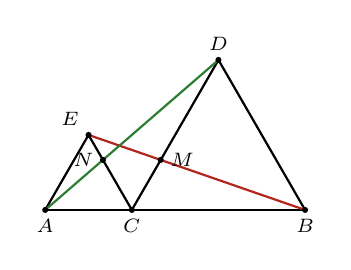
\begin{tikzpicture}[scale=0.55,font=\scriptsize]
\coordinate (A) at (0,0); \coordinate (C) at (2,0); \coordinate (B) at (6,0);
\coordinate (E) at (1,1.732); \coordinate (D) at (4,3.464);
\coordinate (M) at (intersection of E--B and C--D);
\coordinate (N) at ($(C)!0.6667!(E)$);
\draw[thick] (A)--(B); \draw[thick] (A)--(E)--(C) (C)--(D)--(B);
\draw[cThm,thick] (E)--(B); \draw[cRem,thick] (A)--(D);
\foreach \p/\n/\a in {A/A/below,C/C/below,B/B/below,E/E/above left,D/D/above,M/M/right,N/N/left} \fill (\p) circle (2pt) node[\a]{$\n$};
\end{tikzpicture}
\end{LTR}}
\end{tamrin}
\begin{hal}
\textbf{1.} $A$ ، $C$ ، $B$ في استقامية ، إذن $\widehat{ACE}+\widehat{ECD}+\widehat{DCB}=180^\circ$ ، أي $60^\circ+\widehat{ECD}+60^\circ=180^\circ$: \ \bx{\widehat{DCE}=60^\circ}.
\QQ{2} ليكن $r$ الدوران الذي مركزه $C$ وزاويته $60^\circ$ في الاتجاه المباشر:
\begin{itemize}
\item $CB=CD$ و $\widehat{BCD}=60^\circ$: \ $r(B)=D$.
\item $CE=CA$ و $\widehat{ECA}=60^\circ$: \ $r(E)=A$.
\item $CM=CN$ و $\widehat{MCN}=\widehat{DCE}=60^\circ$: \ $r(M)=N$.
\end{itemize}
إذن الدوران المطلوب هو \bx{r\big(C;60^\circ\big)}.
\QQ{3} النقط $B$ ، $M$ ، $E$ في استقامية ، والدوران يحافظ على الاستقامية ، فصورها $D$ ، $N$ ، $A$ \textbf{في استقامية}.\par
والدوران يحافظ على المسافات ، و $r(E)=A$ ، $r(B)=D$ ، إذن \bx{AD=EB}.
\end{hal}

% ------------------------------------------------- 10
\begin{tamrin}{مثلثان قائمان متساويا الساقين وتحويلات}
\RL{0.55}{%
$ABC$ و $ADE$ مثلثان ، كل منهما قائم في $A$ ومتساوي الساقين ، و $H$ المسقط العمودي للنقطة $A$ على $(BC)$ كما هو موضح في الشكل.
\begin{enumerate}
\item بيّن أن المثلثين $ACE$ و $ABD$ متقايسان.
\item بيّن أن المثلثين $ADE$ و $ABH$ متشابهان.
\item استنتج أن: $HB\times ED=AE\times AB$.
\item عيّن التحويلات النقطية التي تحوّل $C$ إلى $B$ (مع التبرير).
\end{enumerate}}{0.42}{%
\begin{LTR}\centering
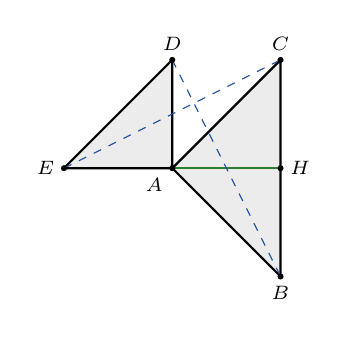
\begin{tikzpicture}[scale=0.55,font=\scriptsize]
\coordinate (A) at (0,0); \coordinate (C) at (2.5,2.5); \coordinate (B) at (2.5,-2.5); \coordinate (H) at (2.5,0);
\coordinate (D) at (0,2.5); \coordinate (E) at (-2.5,0);
\fill[gray!15] (A)--(B)--(C)--cycle; \fill[gray!15] (A)--(D)--(E)--cycle;
\draw[thick] (A)--(B)--(C)--cycle; \draw[thick] (A)--(D)--(E)--cycle;
\draw[cRem,thick] (A)--(H); \draw[cDef,dashed] (E)--(C) (D)--(B);
\foreach \p/\n/\a in {A/A/below left,B/B/below,C/C/above,D/D/above,E/E/left,H/H/right} \fill (\p) circle (2pt) node[\a]{$\n$};
\end{tikzpicture}
\end{LTR}}
\end{tamrin}
\begin{hal}
\textbf{1.} $AC=AB$ و $AE=AD$ ، و $\widehat{CAE}=\widehat{CAD}+\widehat{DAE}=\widehat{CAD}+90^\circ$ ، و $\widehat{BAD}=\widehat{BAC}+\widehat{CAD}=90^\circ+\widehat{CAD}$: \ $\widehat{CAE}=\widehat{BAD}$.\par
الحالة \textbf{(ض ، ز ، ض)}: المثلثان $ACE$ و $ABD$ \textbf{متقايسان} (ومنه $CE=BD$).
\QQ{2} $ADE$ قائم في $A$ ومتساوي الساقين ، فزاويتاه الأخريان $45^\circ$. \ $ABH$ قائم في $H$ ، و $\widehat{ABH}=45^\circ$ (زاوية قاعدة في $ABC$) ، إذن زواياه $90^\circ$ ، $45^\circ$ ، $45^\circ$: المثلثان \textbf{متشابهان}.
\QQ{3} في التشابه تتوافق الزاوية القائمة $A$ في $ADE$ مع $H$ في $ABH$ ، فالوتر $ED$ يوافق الوتر $AB$ ، والضلع $AE$ يوافق $HB$:
\[\frac{ED}{AB}=\frac{AE}{HB}\ \Rightarrow\ \bx{HB\times ED=AE\times AB}.\]
\QQ{4} $AB=AC$ و $H$ منتصف $[BC]$:
\begin{itemize}
\item \textbf{التناظر المحوري} الذي محوره $(AH)$ ($(AH)$ محور القطعة $[BC]$).
\item \textbf{التناظر المركزي} الذي مركزه $H$ ($H$ منتصف $[BC]$).
\item \textbf{الدوران} الذي مركزه $A$ وزاويته $90^\circ$ في الاتجاه غير المباشر ($AC=AB$ و $\widehat{CAB}=90^\circ$).
\item \textbf{الانسحاب} الذي شعاعه $\V{CB}$.
\end{itemize}
\end{hal}

% ------------------------------------------------- 11
\begin{tamrin}{صور أشكال بتحويلات}
$ABCD$ مربع مركزه $O$ وطول ضلعه $4\,cm$ ، و $I$ منتصف $[AB]$.
\begin{enumerate}
\item عيّن صورة المربع $ABCD$ بالتناظر المركزي الذي مركزه $O$.
\item عيّن صورة النقطة $A$ بالدوران الذي مركزه $O$ وزاويته $90^\circ$ (في الاتجاه المباشر ، والمربع $ABCD$ مرتب في الاتجاه المباشر) ، ثم صورة المثلث $OAB$.
\item لتكن $E$ صورة $I$ بالانسحاب الذي شعاعه $\V{AD}$. \ عيّن $E$ ، واحسب $IE$.
\item لتكن $(\mathcal C)$ الدائرة التي مركزها $I$ ونصف قطرها $2$. عيّن صورتها بالتناظر المحوري الذي محوره $(AC)$.
\end{enumerate}
\end{tamrin}
\begin{hal}
\textbf{1.} $O$ منتصف القطرين: $A\mapsto C$ ، $B\mapsto D$ ، $C\mapsto A$ ، $D\mapsto B$: صورة المربع \textbf{هي المربع نفسه}.
\QQ{2} $OA=OB=OC=OD$ والقطران متعامدان: الدوران $r(O;90^\circ)$ يحوّل $A\mapsto B$ ، $B\mapsto C$. \ صورة المثلث $OAB$ هي المثلث $OBC$ (يقايسه).
\QQ{3} $\V{IE}=\V{AD}$: \ $E$ منتصف $[DC]$ (لأن الانسحاب يحافظ على المنتصف ، وصورة $[AB]$ هي $[DC]$) ، و \bx{IE=AD=4\,cm}.
\QQ{4} التناظر المحوري يحافظ على الأطوال: صورة الدائرة هي الدائرة التي مركزها $I'$ صورة $I$ ونصف قطرها $2$. \ $(AC)$ محور تناظر للمربع يحوّل $B$ إلى $D$ ، إذن صورة $I$ (منتصف $[AB]$) هي $I'$ منتصف $[AD]$.
\end{hal}

% =====================================================================
\section{صحيح أم خطأ ، اختيار من متعدد}
% ------------------------------------------------- 12
\begin{tamrin}{صحيح أم خطأ}
أجب بصحيح أو خطأ مع تعليل الإجابة:
\begin{enumerate}
\item إذا كان $[AB]$ و $[CD]$ قطرين في دائرة فإن الرباعي $ACBD$ مستطيل أو مربع.
\item $ABC$ مثلث قائم في $A$ حيث $BC=2AB$. لا يمكن حساب قيس الزاوية $\widehat{ACB}$ بهذه المعطيات فقط.
\item المثلث الذي أطوال أضلاعه $6$ ، $8$ و $10$ قائم.
\item مثلثان لهما زاويتان متقايستان مثنى مثنى متقايسان.
\item الدوران يحافظ على المسافات وعلى التوازي.
\item إذا كان مثلثان متشابهين بنسبة $3$ فإن مساحة الثاني ثلاثة أضعاف مساحة الأول.
\item صورة مستقيم بانسحاب مستقيم يوازيه.
\end{enumerate}
\end{tamrin}
\begin{hal}
\textbf{1.} \textbf{صحيح:} القطران متقايسان (طول كل منهما $2r$) ومتناصفان (في $O$) ، فـ $ACBD$ مستطيل (ويكون مربعاً إذا كانا متعامدين).
\QQ{2} \textbf{خطأ:} $\sin\widehat{ACB}=\dfrac{AB}{BC}=\dfrac12$ ، إذن $\widehat{ACB}=30^\circ$.
\QQ{3} \textbf{صحيح:} $6^2+8^2=36+64=100=10^2$.
\QQ{4} \textbf{خطأ:} هما متشابهان فقط (مثلاً مثلثان متقايسا الأضلاع ضلعاهما $1$ و $2$).
\QQ{5} \textbf{صحيح:} الدوران تقايس.
\QQ{6} \textbf{خطأ:} المساحة تُضرب في $k^2=9$.
\QQ{7} \textbf{صحيح.}
\end{hal}

% ------------------------------------------------- 13
\begin{tamrin}{اختيار من متعدد}
اختر الإجابة الصحيحة الوحيدة مع التعليل:
\begin{enumerate}
\item نقطة تلاقي متوسطات مثلث هي:
\ABC{مركز الثقل}{المركز القائم}{مركز الدائرة المحيطة}
\item $ABC$ قائم في $A$ ، $AB=3$ و $AC=4$. طول المتوسط $[AI]$ ($I$ منتصف $[BC]$) هو:
\ABC{$5$}{$2{,}5$}{$3{,}5$}
\item $(MN)\parallel(BC)$ ، $AM=2$ ، $AB=6$ و $BC=9$. الطول $MN$ هو:
\ABC{$3$}{$4{,}5$}{$27$}
\item مثلث مساحته $12\,cm^2$ ، صورته بتشابه نسبته $\dfrac12$ مساحتها:
\ABC{$6\,cm^2$}{$24\,cm^2$}{$3\,cm^2$}
\item التحويل الذي لا يحافظ على اتجاه الزوايا هو:
\ABC{الانسحاب}{التناظر المحوري}{الدوران}
\item $ABC$ قائم في $A$ ، $BC=10$ و $\widehat B=60^\circ$. الطول $AB$ هو:
\ABC{$5$}{$5\sqrt3$}{$10\sqrt3$}
\end{enumerate}
\end{tamrin}
\begin{hal}
\textbf{1.} (أ). \quad \textbf{2.} (ب): $BC=5$ ، والمتوسط المتعلق بالوتر يساوي $\dfrac{BC}2$. \quad \textbf{3.} (أ): $MN=\dfrac26\times9=3$.
\QQ{4} (جـ): $\Big(\dfrac12\Big)^2\times12=3$. \quad \textbf{5.} (ب). \quad \textbf{6.} (أ): $AB=BC\cos60^\circ=5$.
\end{hal}

\end{document}
